% RECOMMENDED %%%%%%%%%%%%%%%%%%%%%%%%%%%%%%%%%%%%%%%%%%%%%%%%%%%
\documentclass[graybox]{svmult}

%\usepackage{mathptmx}       % selects Times Roman as basic font
\usepackage{helvet}         % selects Helvetica as sans-serif font
\usepackage{courier}        % selects Courier as typewriter font
\usepackage{parskip}

% my stuff
% \usepackage{draftwatermark}
\usepackage{dirtytalk}
\usepackage{hyperref}

\usepackage{type1cm}          % activate if the above 3 fonts are
                              % not available on your system

\usepackage{makeidx}          % allows index generation
\usepackage{graphicx}         % standard LaTeX graphics tool
                              % when including figure files
\graphicspath{{Figures/}}
\usepackage{multicol}         % used for the two-column index
\usepackage[bottom]{footmisc} % places footnotes at page bottom

% see the list of further useful packages
% in the Reference Guide

\makeindex             % used for the subject index
                       % please use the style svind.ist with
                       % your makeindex program

%%%%%%%%%%%%%%%%%%%%%%%%%%%%%%%%%%%%%%%%%%%%%%%%%%%%%%%%%%%%%%%%%%%%%%%%%%%%%%%%%%%%%%%%%

\begin{document}
%\SetWatermarkText{DRAFT}
%\SetWatermarkScale{1}
\title*{KTH Formula Student: Principles and Statute}
\author{Management Team - 2018}
\maketitle
\section{Core Values}
\label{sec:1}

\subsection*{Our Vision}

\begin{center}
\Large{{\textbf{To be the best Formula Student team in Sweden.}}}
\end{center}
 
\subsection*{Our Mission}
\large{{The aim of KTH Formula Student is to build a \textbf{fast and robust electric and driverless racing cars} that will join the \textbf{best European Formula Student competitions} every year.

KTH Formula Student focus its efforts in the development of innovative and \textbf{cutting-edge technologies} in synergy with KTH and partner companies.

The \textbf{Team} always represents the first assets and priority of KTH Formula Student. The Team is composed by motivated and ambitious KTH students with \textbf{diverse backgrounds} from both Bachelor and Master degrees. KTH Formula Student promotes the Team development in both \textbf{learning outcome} and \textbf{social cohesion}.

KTH Formula Student achieve these goals with a \textbf{structured and clear organization} and persistent \textbf{self-improvement}, mainly based on a solid \textbf{knowledge-transfer} through the years and \textbf{continuity} both in the Team and in the partnerships.
}}


\subsection*{Key Words}
\begin{itemize}
    \item \textbf{The Product}
    \begin{enumerate}
        \item Fast and Robust car
        \item Best competitions
        \item Innovative solutions
    \end{enumerate}
    \item \textbf{The Team}
    \begin{enumerate}
        \item People first, results driven
        \item Diverse background
        \item Learning outcome
        \item Friends
    \end{enumerate}
    \item \textbf{The Organization}
    \begin{enumerate}
        \item Structured and clear
        \item Knowledge transfer
        \item Continuity
    \end{enumerate}
\end{itemize}

\subsection*{Mission details}
\begin{itemize}
    \item \textbf{The Product}:
    \begin{enumerate}
        \item 	\textbf{Fast and Robust car:}
        
        Plan the works in order to provide a testable car earlier in the year able to guarantee robustness and performances. Continuity, knowledge-transfer and structured organization will provide new tools to respect deadlines.
    
        \item \textbf{Best competitions}
        
        A team with passionate Bachelor students (up to 50$\%$) will provide the required continuity to achieve higher results during the qualifications. If we achieve this, we will create a great brand.
        A great brand is a fundamental step towards the creation of a great team.

        \item \textbf{Innovative solutions}
        
        A solid knowledge transfer and competition successes will give us the knowledge and the resources (both from partners companies and KTH) to achieve more ambitious technological solutions.
    \end{enumerate}
    \item \textbf{The Team}:
    \begin{enumerate}
        \item \textbf{People first, results driven}
        
        We believe that a clear and structured organization will provide higher outcomes of our efforts. Examples of tools: Job Description, clear personal responsibilities (“Deliver on time, no surprises!”) with well-defined projects (QQTR), organization charts, effective project management and clear performance evaluation.
        
        \item \textbf{Diverse background}
        
        Diverse background means teams composed both Bachelor and Master students from different study areas. This will help with both non-technical solutions, team organization and qualifications.

        \item \textbf{Learning outcome and Friends}
        
        The priority is always to provide the best experience to team members. Both in the learning outcome and in social activities. We want to create a great place to work.
    \end{enumerate}
    \item \textbf{The Organization}:
    \begin{enumerate}
        \item \textbf{Structured and clear}
        
        To create an effective organization training and knowledge are required. This means that all the members and management team (in particular) have to improve their project and group management skills and be aware of how an organization works.
    
        \item \textbf{Knowledge transfer and continuity}
    
        In order to achieve all these goals continuity and knowledge transfer are fundamental. This has to be implemented both through a structured training for the new entries and workshops by former members.
    \end{enumerate}
\end{itemize}

\section{Organization Structure, Roles and Processes}
\label{sec:2}

\begin{figure}
    \centering
    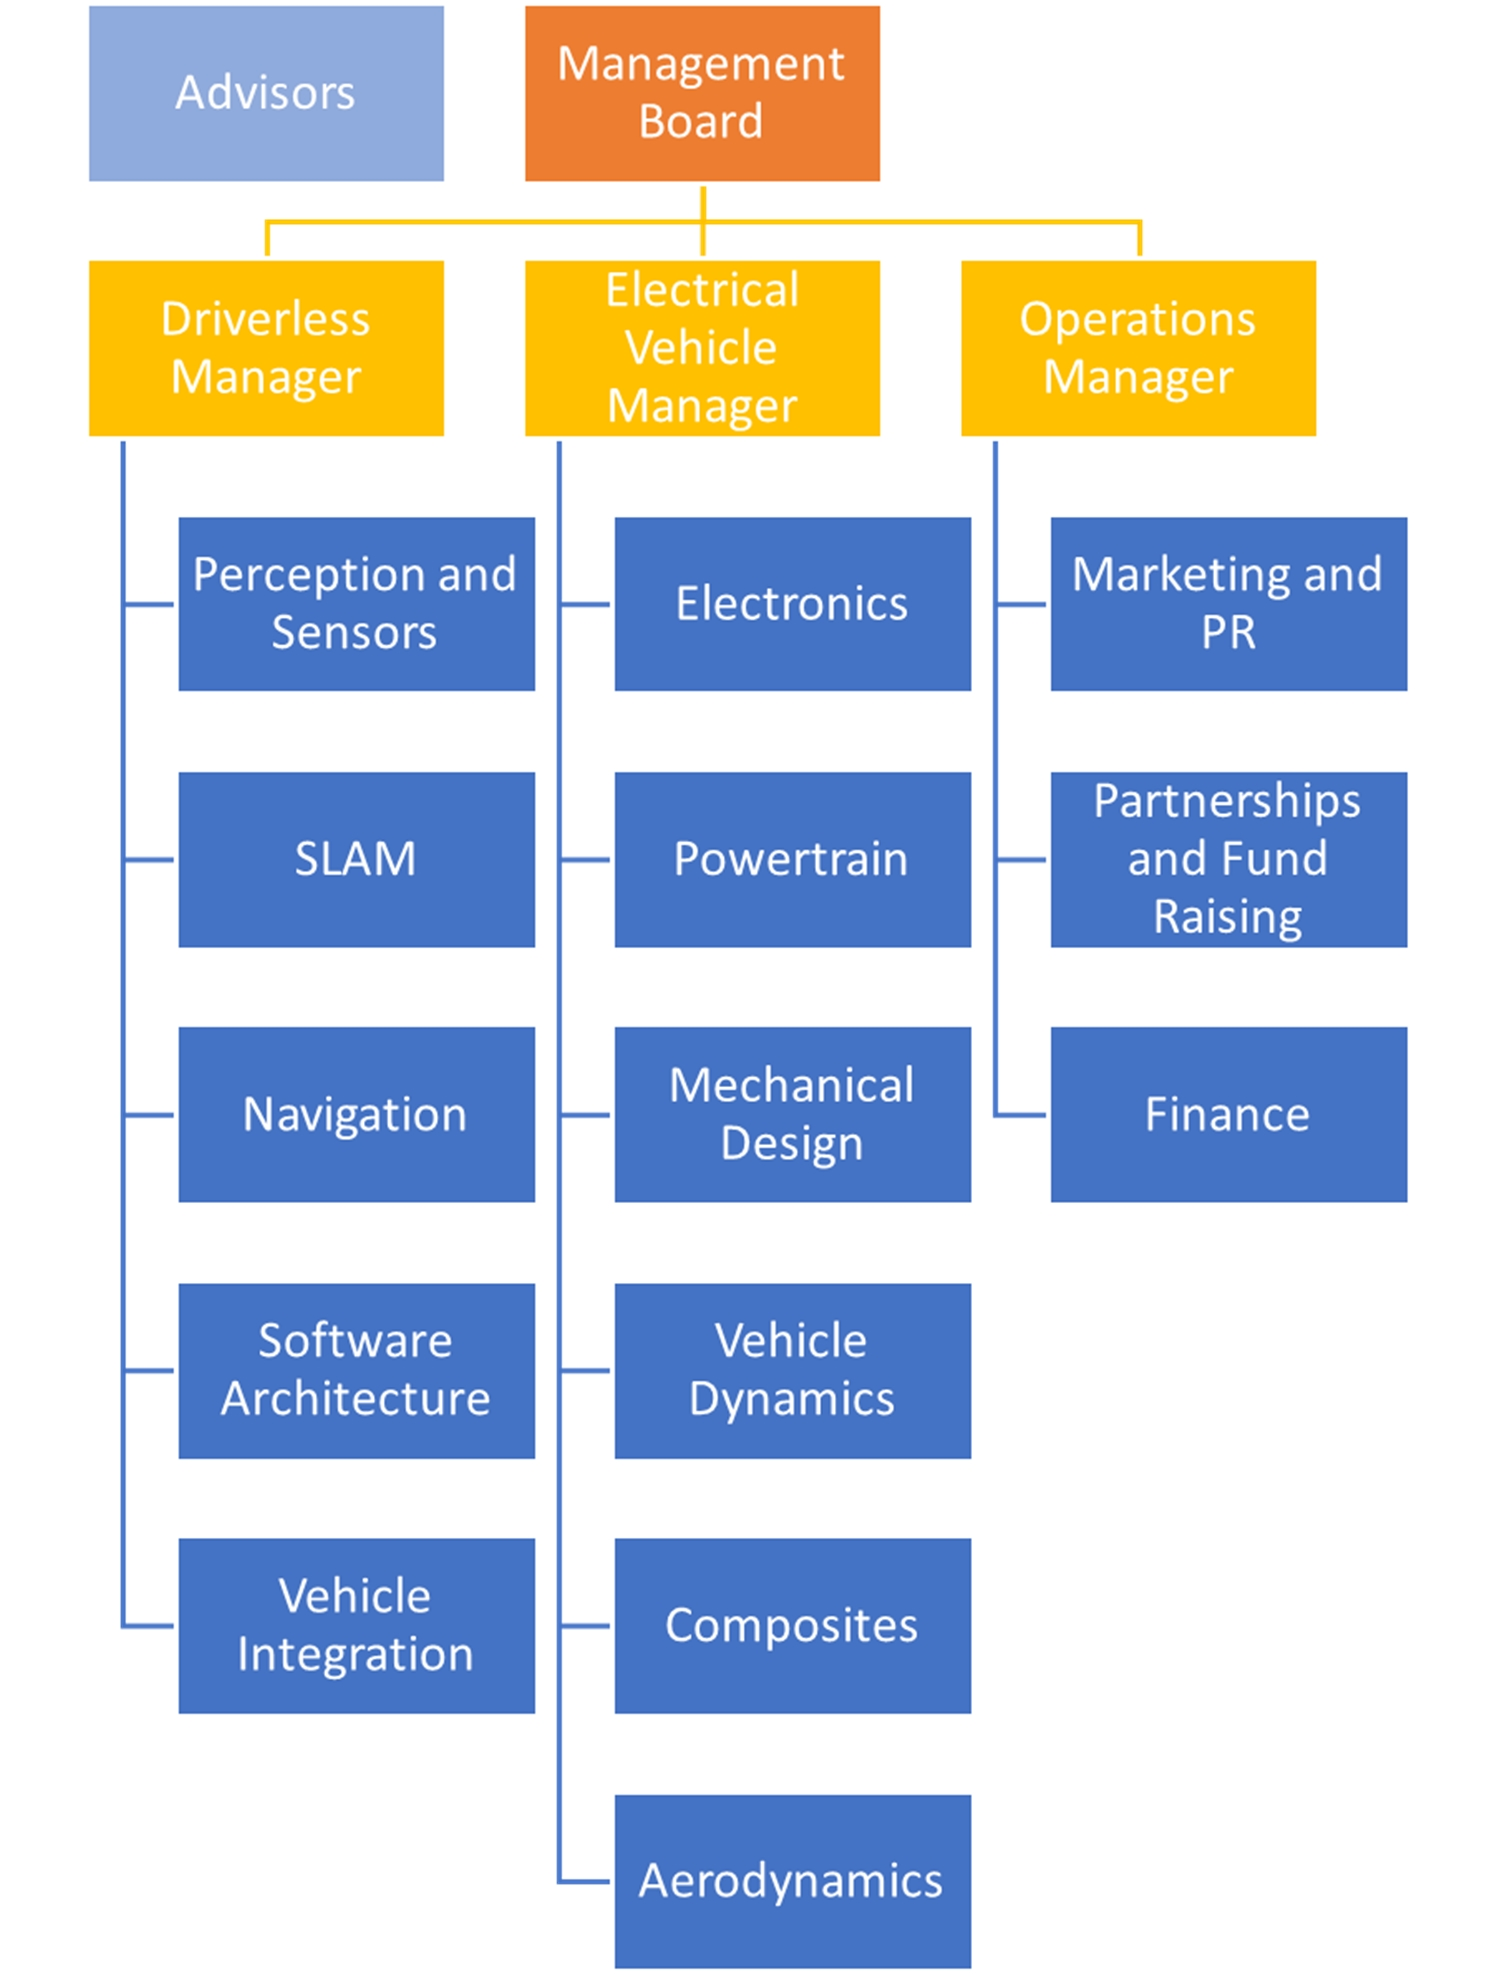
\includegraphics[scale=.60]{organigramma.jpg}
    \caption{Organization chart. Note: Marketing and PR is renamed as "Communication and Marketing"}
    \label{fig:chart}
\end{figure}

\subsection{Management Board}
The management board is responsible for the overall organization operations, decisions and success of the overall team. The management board represents the head and final approver of the whole KTH FS team. The management board is composed by the three team managers and by all the group leaders. The management board has to work towards the realization of the Core Values expressed in the Vision and Mission.

\subsection{Managers}
The managers coordinate the three departments: Driverless, Electrical Vehicle and Operations. They do not take part in the technical development in first person, but discuss and approve the design the overall technical plan with the support of the group leaders.
The managers have important role in project management and communication between the groups both in the same department and in transversal works through different departments.
The managers also has the role of representing the team in front of companies, university, conferences and other events.
They have responsibilities in fund raising and company relationships in collaboration with the Operations department.
Each manager is the first responsible for her/his department operations, organization and success of the department projects.

\subsection{Groups}
Each group defines an area of expertise and usually also an ensemble of related projects that will be handled within the group itself. Members with similar interests, knowledge and responsibilities compose each group. All the groups have a representative member that will be defined as Group Leader and will join the management board. The group leader beside the technical work will have management and communication responsibilities.
The number of members of a group is variable but has to be at least three people and at most seven. Division and merging of groups will be handled accordingly by the department manager and management board. The reasons for this limitations are the following: too large group will hardly have a frequent and effective communication. Moreover, the Group Leader would require to invest too much time for an effective team management.
On the other side, too small group might cause isolation from the rest of the team and consequently lack of communication and knowledge transfer. Moreover, the success of the overall team would be too much dependent to the result of very few members.

\subsection{Group Members}
\subsubsection{Role and Contribute: Job Description}
All the people that successfully pass the recruitment selection process become KTH FS Members.
Members have a clear and exhaustive Job description that specify exactly what are the role, contribution and responsibilities.
Any major changes and customization to role, contribution and responsibilities need to be clearly reported in the job description.
The job description need to be discussed between the member and the group she/he belong to. Moreover the job description need to be approved by relative Department Manager.
The member define with the group what activities, projects and responsibilities he/she want to follow and invest time. Implicitly this also define what activities the member do not need and should not follow. It is crucial for both of the parties (team and member) to have a clear and common view of the role and contribution. For the member that is important in order to have guarantee that all the invested time will be always related with his/her area of interest and expertise, i.e. the reason why he/she joined in the first place.
For the organization a clear role for members is fundamental both for a balanced and control work division and for a fair evaluation performance.
\subsubsection{Time and priorities}
The time and efforts invested in the project is variable, flexible, but consistent during the year. The performance though, will always be related with the quality of results obtained with respect to the result expected (see RACI project in \ref{sec:3}). 
\subsubsection{Member Outcome}
The organization has to provide and guarantee a concrete and effective outcome for all the members.
\begin{itemize}
    \item \textbf{Learning outcome}: the organization set as first and most important outcome for the member a concrete and effective learning process. This will be delivered with organized knowledge transfer and through the organization resources: equipment, services, sponsors and companies courses and meetings, professors and university collaboration.
    \item \textbf{Social Cohesion}: the organization will always work towards the creation of a positive and inclusive environment that promote the social cohesion and sense of belonging to the group.
\end{itemize}
The two objective should always be compatible and mutual supported.
During the selection process the outcome should be clearly stated to the candidates. At the same time, their understanding and belief in the organization Vision and Mission will be the most important aspect taken into account for the recruitment.


\subsection{Group Leaders}
The responsibilities of the group leader:
\begin{itemize}
\item \textbf{Technical}: As all the other members, the primary role of the GL is the technical development. The GL will invest the majority of her/his time accomplishing technical tasks in first person. Moreover, as requisites, the GL has a robust knowledge about the group specific technical area. The GL is perfectly aware of what are the responsibilities and role of the group she/he leads. The GL knows how her/his group is linked with others groups and how the contribution of the group affect the overall project. To achieve this aim, the GL is confident with other technical areas and with the organization structure. As every other member in the team, the GL is involved in first person in projects and technical tasks. The role of GL is not directly related with successful technical achievements, but mostly with personal predisposition.
\item \textbf{Management}: the GL invest a significant part of her/his time to managerial activities. In order to achieve these tasks successfully, the GL receives specific training in team and project management. The amount of time required to be invested in management activities is related parameters such as the number of members in the group and the role of the group in the team (the time invested in management should roughly belong to 20$\%$ up to 40$\%$).
\end{itemize}

\subsubsection{Focus: Management responsibilities of group leader}
\begin{itemize}
\item \textbf{Management Board}: the GL joins the Management Board and its activities with periodic meetings and additional activities.
\item \textbf{Group management}: the GL invests time in the group and its members to guarantee the best experience, learning outcome and social cohesion for everybody as expressed in the Core Values. The GL guarantees a fair distribution of the responsibilities and projects allowing everybody to improve and enjoy their activities. Moreover, the GL knows how to handle wisely possible conflicts.
\item \textbf{Project management}: the GL knows how to deliver and handle projects within QQTR (Quality, Quantity, Time and Resources). The GL is confident in project management tools, techniques and best practices.
\end{itemize}
    
\subsection{Manager and Group Leader recruitment}
The selection of GLs and Managers is a decision taken as a result of a constructive discussion in the team through all the involved members. The criteria taken in consideration are: experience and involvement in the team (primary requirement) and personal predisposition to management and transversal activities. In any way the role has to be used as reward for successful technical results or considered as a promotion to an higher level of involvement (since the high involvement has to be shared through all the team members independently to the covered position).

\subsubsection{Group Leader recruitment}
The choice of a new group leader is the result of an open discussion (preferably with no elections) within the group, the former Group Leader and the Department Manager. The final decision then will be briefly discussed and approved by the Management Board.

\subsubsection{Management recruitment}
The selection of the Managers will be primarily handled by the Group Leaders of the relative department, the former Manager and then discussed and approved by the Management Board.
If any of these processes fails to find a new Manager or GL, the responsibility come to the Management Board.

\subsubsection{Timing for management and GLs recruitment}
The choice of the new figures should be done preserving continuity and knowledge transfer during the passage. This can be performed initially trough collaboration between the current GL/manager and the next one, then with mentoring from the former GL/manager to the new one.

\subsection{Duration of the GLs and Management roles}
The normal duration of Managers and GLs could vary from a minimum of 6 months charge and can be renewed once with a maximum of 1 year.

\subsection{Advisors}
Alumni and other experienced profiles that help the organization (both in technical and management fields) would join the Advisors. The Advisors have no decision or technical responsibilities, they cannot take part of projects with the role of Responsible or Approver, but can be referred as Collaborators and Informee. They are always welcome to join the activities of the team both in the technical and social development. Their presence and constant involvement in the team represent a great added value and resource for the overall team. The involvement of Advisors should be encouraged and supported.

\section{Project Management}
\label{sec:3}

\subsection{How to create project groups}
The projects are handled using the Responsibility Matrix: RACI model (or equivalent). 
In particular, each project needs to have:
\begin{enumerate}
\item \textbf{Responsible} (unique): the member that take the responsibility for the successful completion of the project.
\item \textbf{Approver} (at least one): The ones ultimately answerable for the correct and thorough completion of the deliverable or task, and the one who delegates the work to the Responsible.
\item \textbf{Collaborators}: They support and advise the project responsible. If they have operative tasks they should also have clear responsibilities in the project. The Approver of this sub-project is the Responsible of the original project.
\item \textbf{Informee}: people that has no active role within the project completion, but they need to be constantly informed about the project developments.
\end{enumerate}
Each role need to be properly informed and involved in the project development. Moreover, the overall task division has to be properly documented. You cannot cover more than one role in the same project.
Nested projects are allowed, but a proper documentation and communication need to be implemented.

For other info: \href{https://en.wikipedia.org/wiki/Responsibility_assignment_matrix}{Wikipedia Link -  Responsibility Matrix}


\subsection{How to deliver project}
\subsubsection{QQTR: Quality, Quantity, Time and Resources}
The project has to be delivered with clear QQTR determined through discussion between the Approver and the Responsible (and Collaborators).
Mandatory to specify each single aspect, with particular care to set ambitious, but feasible deadlines (Time). Exactly specify the Resources, such as literature, collaborators, professors, advisors and tools (i.e. competition rules book). Clearly state the expected Qualitative and Quantitative performances as well.
The QQTR has to be properly documented.
(more info in Vision and Mission document and internet \href{https://mikecardus.com/shared-language-of-goal-setting-will-ensure-goals-are-understood/}{Goal Setting Link})

\subsubsection{Deliver On Time No Surprises: How to handle deadlines and execution}
The project are handled with “Deliver On Time, No Surprises”. This means that there is no control by the Approver on the daily activity of the Responsible. The Responsible is aware that in case of problems he/she will never receive any judgment (or evaluation) on mistakes or inconveniences. At the same time he/she has the \textbf{responsibility and duty} to inform the Approver as soon as possible of any circumstance that may threaten the designed QQTR. The project manager (Approver) becomes in this process the primary support for the team member helping them to reach their goals.
In this case, the Approver and Responsible work together on a new and better solution defining new QQTR.

In this process, there is \textbf{no judgment} of the mistakes of the people, but instead positive encouragement toward common goals (this management style takes the name of “Deliver on time, no surprises!”).

\begin{svgraybox}
When can the Deliver On Time, No Surprises might fail?
\begin{enumerate}
\item If the QQTR is unclear or not discussed and approved both by Responsible and Approver.
\item If the Responsible is afraid to be judged due to mistake or problems. The Approver then needs to create the optimal environment to allow the Projects Responsible to be open about the project developments.
\end{enumerate}
\end{svgraybox}

\subsection{How to define the roles in team projects}
\subsubsection{Projects division}
\begin{enumerate}
\item \textbf{Vertical Project}: projects completely (or almost completely) handled within the same group. Usually they are part of bigger projects. The Responsible belongs to the group and the Approver is the Group Leader (if not directly involved) or the relative department Manager.
\item \textbf{Transversal Project within same department}: Projects that involve many group belonging to the same department. In this case, the Responsible is chosen within the members of the involved groups and the Approver is the department Manager.
\item \textbf{Transversal Project across departments}: Projects that involve groups in different departments. The Approver is chosen among the Managers of the involved Department.
\item \textbf{Macro Projects}: Projects that involve high number of members involved with extraordinary tasks (such as qualification, testing or event organizations). In this case the Approver is the Management Board.
\item \textbf{Management Projects}: Projects that involve one or more Managers as Responsible. The Approver is the Management Board.
\end{enumerate}

\section{Focus: Operation Department}
\label{sec:4}
\subsection{Core Values}
\subsubsection*{Vision}
\subsubsection*{Mission}
\subsection{Department groups}
\begin{itemize}
    \item \textbf{Communication and Marketing}
    \begin{itemize}
        \item \textbf{Responsibility}: responsible for the communication of KTHFS, promotion of the brand of KTHFS and related social activities.
        \item \textbf{Activities}: Mainly related to brand positioning, social media lead acquisition, business and academic event organization for both members and external profiles.
        \item \textbf{Knowledge}: Social Media, Marketing, Event organization, Brand Positioning, Media Creation
    \end{itemize}
    \item \textbf{Partnerships and Fund Raising}
    \begin{itemize}
        \item \textbf{Responsibility}: Responsible for the acquisition, management and development of current partners (university, companies, investors, organizations). Responsible for effective fund and resources raising for the team activities.
        \item \textbf{Activities}: Continuous communication with departments and Finance in order to acquire new sponsors and partners. Deep connection with Marketing and PR for positive relationship with current partners. 
        \item \textbf{Knowledge}: Business Economics, Business Strategy, Business Management and Investments. Experience/Interest in company, university and organizations relationship.
    \end{itemize}
    \item \textbf{Finance and Business Development}
    \begin{itemize}
        \item \textbf{Responsibilities}: Handling of the economic, finance, balance and budgets of the whole organization. Responsible for business planning and strategy for development. 
        \item \textbf{Activities}: handle the balance sheet with income from partnership and university, evaluating and organizing the investments and expenses for the organization activities.
        \item \textbf{Knowledge}: Business Management, Strategy and Economics. Experience/interest in finance.
    \end{itemize}
\end{itemize}
\subsection{Recruitment Process 2018}
TBD!

\section{Focus: The Electrical Department}
\label{sec:5}
\subsection{Core Values}
\subsubsection{Vision}
\subsubsection{Mission}
\subsection{Department groups}
\subsection{Recruitment Process 2018}
TBD!

\section{Focus: The Driverless Department}
\label{sec:6}
\subsection{Core Values}
\subsubsection*{Vision}
\begin{center}
\large{{\textbf{To be the best FS driverless team in North Europe.}}}
\end{center}
\subsubsection*{Mission}
Every year the Driverless department deliver a fully autonomous vehicle able to join the \textbf{best European FS competitions}.

Every year we will rely on the car built by the Electric Vehicle department for the previous competition.
We will offer the \textbf{most robust and innovative driverless technology}.

Our team is composed by bright, passionate and reliable technology enthusiasts, with passion in the field of Robotics, AI and ML.

We believe in the synergy of deep connection with KTH and partner companies. We publish and share our works with scientific community over the boundaries of the FS competition. We aim to become a \textbf{reference and a laboratory for our university} and its students.

We are and we will remain a fundamental pillar of KTH Formula Student, \textbf{we strongly believe in the synergy with the other departments} towards the fulfillment of our common Vision and Mission. 

\subsection{Department groups}
\begin{itemize}
	\item \textbf{Perception}
	\begin{itemize}
		\item \textbf{Responsibility}: The Perception group has the responsibility for all the perception pipeline of the system, starting from the physical sensors HW to the software elaboration, algorithms, sensor fusion and finally the refined output to be sent to the SLAM group. The perception group is the first responsible for the sensors: 3D-Lidar and Zed Stereo Camera.
		\item \textbf{Activities}: Mainly focus related to computer vision, machine learning algorithms, sensor fusion and code development and perception pipeline testing.
		\item \textbf{Knowledge}: Python/C++ coding, ANN and ML, data preprocessing, CV and Image Analysis, ROS, Tensorflow/Pytorch.
	\end{itemize}
    
	\item \textbf{SLAM: Localization and Mapping}
	\begin{itemize}
		\item \textbf{Responsibility}: The SLAM (Simultaneous Localization and Mapping) group has the responsibility for all the SLAM pipeline, i.e. the system that given the sensor data provide an estimation of the surrounding map and pose of the robot. This group has to be in close relationship both with perception (for a correct input management) and with Navigation group (for the outputs requirements). The SLAM group is also responsible for the sensors: IMU and wheel encoders. 
        \item \textbf{Activities}: Mainly focus on SLAM algorithms and architecture, ROS, virtual environment simulations and tests.
		\item \textbf{Knowledge}: Robotics, Python/C++ coding, ROS, SLAM, EKF, Particle Filters, software architecture (due to the central position in the pipeline, transversal knowledge will be learned).
	\end{itemize}

	\item \textbf{Navigation}
	\begin{itemize}
		\item \textbf{Responsibility}: The Navigation group is responsible for all the car navigation pipeline, starting from the path finding and planning, trajectory generation and tracking and finally autonomous car controls. This group, given the input from the SLAM group, will provide the optimal trajectory updated in real time and send this output to the dSpace for the atual vehicle actuation.
		 \item \textbf{Activities}: Focus on control and navigation algorithms development and tests. 
		\item \textbf{Knowledge}: Python/C++/Matlab coding, ROS, AI (planning), Robotics, Controls and MPC.
	\end{itemize}

	\item \textbf{Software Architecture}
    \begin{itemize}
		\item \textbf{Responsibility}: The Software Architecture group is responsible for the general software architecture of the DV system. Responsible for choice and configuration of the computer specs and layout. Responsible for SW safety, faults detection, simulations, software optimization and configurations. This group is a constant and organized support for the other software group.
		\item \textbf{Activities}: Code development and debug, general ROS architecture design, technical coordination of other systems merging.
		\item \textbf{Knowledge}: Python/C++ coding, ROS, Computer Science, Robotics, SW confident, SLAM, Sensor Fusion architecture.
	\end{itemize}

	\item \textbf{Vehicle Integration}
	\begin{itemize}
		\item \textbf{Responsibility}: This group is responsible for DV optimal HW system integration   with the vehicle. Responsible for networking and communication protocol, dSpace programming, electric and electronics system, DV actuators development, HW safety issues and rule compliance. The VI group is responsible for the correct handling of the Navigation input and elaboration towards actual car control. Responsible for bridge communication and collaboration and outsourcing with other groups in EV department regarding HW developments. 
		\item \textbf{Activities}: Actuators design, electronics and network design, low-level controls (dSpace) for DV system. Communication, coordination and teamwork with EV.
		\item \textbf{Knowledge}: Mechanical Design, Electric Drives, Electronics, Networking, Matlab/Simulink, dSpace. Effective communication, project management and teamwork.
	\end{itemize}
\end{itemize}

(TBD: details of job descriptions – 1 page each)

\subsection{Recruitment Process 2018}

The extensive recruitment phase start in early September.
All students are welcome to join the recruitment process (both bachelor and master students).
The selection process has to be fair, respectful and transparent: diversity and unbiased targeting has to be guaranteed.
Different requirements are specified according to application macro groups: Software or Vehicle Integration.

Despite the interviewing will start in early September, the communication will start in the second half of August.

\subsection{Communication and Marketing}

The Driverless team will follow two parallel paths for communication and marketing finalized to the new year recruitment:
\begin{itemize}
    \item General communication
    \item Targeted communication
\end{itemize}

\subsubsection{General Communication}
The General communication is mainly focused on the production and sharing of media material for social media. The material should concern driverless, robotics and AI technology, developments and KTH-FS environment.
A small social media payed plan or Google Ad-Word can be considered too.
For an effective sharing of this contents social media targets has to be identified such as Facebook groups and pages that are likely to be used by possible candidates.
In parallel with the creation of such material, fliers distribution and other means can be considered.


\subsubsection{Targeted communication}
The targeted communication is focused on the identification of best candidates profile. The targets should not be disguised as requirements, but instead as courses and programmes attended by possible candidates.

Students, professors and coordinators of these programmes and courses should be contacted and informed about our project and relative opportunities.
This will be done with fliers distributed out of the classes, introduction speeches during lessons, mails sent by professors and program coordinators.

\begin{itemize}
  \item \textbf{Target Programmes}
  
  Courses that likely have potential members, not to be considered as exclusive principle.
  
  \begin{enumerate}
    \item System Control and Robotics
    \item Machine Learning
    \item Computer Science
    \item Embedded Systems
    \item Mechatronics
    \item Vehicle Engineering
    \item ...
  \end{enumerate}

  \item \textbf{Target Courses}
  
  Courses in P1 and P2 to target for recruitment, not required for access.
  
  \begin{itemize}
    \item \textbf{Period 1}
    \begin{enumerate}
      \item Robotic and Autonomous Systems
      \item Modelling of Dynamical Systems
      \item Project Course in Data Science
      \item Artificial Intelligence
      \item Machine Learning
      \item Model Predictive Control
      \item ...
    \end{enumerate}
    \item \textbf{Period 2}
    \begin{enumerate}
      \item Computer Vision and Image Analysis
      \item Applied Estimation
      \item Nonlinear Control
      \item Reinforcement Learning
      \item Machine Learning Advanced
      \item Automatic Control - Project Course
      \item ...
    \end{enumerate}
  \end{itemize}
\end{itemize}

\subsection{Driverless Recruitment process}
\subsubsection{New year recruitment}

Through a \textbf{Google Form}, we receive candidate data and schedule interviews.

\begin{enumerate}
  \item \textbf{First Phase: Minimal Requirements (1 week)}
  Requirements:
  \begin{itemize}
    \item For everybody:
    \begin{enumerate}
      \item Interested in Driverless
      \item Good in teamwork
      \item Highly reliable
    \end{enumerate}
    \item For Software tracks:
    \begin{enumerate}
      \item Confident in coding (C++/Python/Matlab)
      \item Passionate in robotics or machine learning topics
    \end{enumerate}
    \item For Vehicle Integration track:
    \begin{enumerate}
    	\item Passionate in robotics and driverless cars.
    	\item Confident in Simulink, electronics, electric drives, CAD and controls.
        \item Sufficient in coding and Algorithms (C++/Python/Matlab)
    \end{enumerate}
  \end{itemize}


No hard selection is performed in Phase 1, the aim of this interview is to present quickly the system and organization and verify the correctness of the minimal requirements through specific questions and examples (10 min of interview). The candidate can (should) support her/his application with CV, LinkedIn, Transcripts and GitHub profile or equivalent.
If the minimal requirements are satisfied the candidate can access to the second phase.
If the candidate show much higher knowledge, the interviewer will communicate the candidate profile to the rest of the group. With the approval of the group leader and manager a second longer and more technical interview can be settled in order to evaluate a faster recruitment procedure (see section about Cherry Picking or In-Itinere process).

\item \textbf{Second phase: General Training (1 week)}
\begin{itemize}
\item \textbf{For SW}: Old members provide one extensive lecture for each DV group (Perception, SLAM, Navigation and VI) providing a general knowledge and relative literature.
\item \textbf{For VI}: Old members provide one extensive lecture for: DV-software, DV-VI, VD, Electronics providing a general knowledge and relative literature.
\item \textbf{Everybody}: DV manager extensive lecture about Project Management and Organization Structure and KTH-FS core values and Principles.
\end{itemize}

\item \textbf{Third phase: track selection and specific training (2 week)}
\begin{itemize}
\item \textbf{For SW}:
The candidates choose at least one track to follow (preferably two). Each GLs lead a 2 week crash course about one of the major tracks: Perception, SLAM and Navigation. The crash course does not need to be designed by the group, but instead it should refer to a series of online available material and courses that can be studied and presented together. See Training Process Outline.
\item \textbf{For VI}:
Old members provide 2 weeks crash courses about VI and EV bridges activities. This training will be provided by both DV and EV members, and coordinate by VI members.
\item \textbf{For everybody}: 
All tracks must include at least one \textbf{personal project submission} and final oral discussion/interview with GLs and DV manager.
\end{itemize}
\end{enumerate}

The candidates that successfully pass the third phase are assigned to the 5 DV groups and effectively become new KTH FS members.
The candidates that did not pass the final examination due to not sufficient results can ask for a re-exam presenting a new project chosen with the examiner and new interview within one week.
The candidates that did not present the assignments or skipped two or more lectures cannot apply for the retake.

Other forms of recruitment:
\begin{itemize}
\item \textbf{In-itinere process}:
The process will have the same (or higher) requirements, but there will be no lectures taken by the old members, the course outline will be available online though. This process have higher requirements than the standard recruitment process. The process is then structured as follow: one short interview for minimal requirement and group presentation. One long interview a week later with small project submission and discussion with GLs and DV manager.
This process hold also for current KTH members that would like to join the driverless team (only if they are not already considered for Cherry Picking).

\item \textbf{Cherry picking}:
In rare case of advanced knowledge and particularly brilliant profiles, the DV Manager in agreement with all GLs can hire new members without process.

\item \textbf{Membership after university/thesis – project}:
In this case the membership will be evaluate according to the passion and performances (social and technical) showed during the university project regarding KTH FS driverless.
\end{itemize}

\subsubsection{Training Process Outline}
The examiners provide a complete outline of the training process with topics and exhaustive resources (books, online courses, slides). The selection process has to be explained and published in details as well. This can be done on specific GitHub or website pages.
The description should include:
\begin{enumerate}
\item \textbf{Prerequisites}: necessary knowledge to start the training. This knowledge will not be provided during the training phase.
\item \textbf{Evaluation subjects}: knowledge that receive proper introduction during training phase and will be subject of recruitment evaluation.
\item \textbf{Expectations}: Desired level of knowledge after training phase.
\item \textbf{Road-map}: Path towards desired goals (i.e. crash course literature and syllabus).
\item \textbf{Evaluation}: Clear evaluation criteria both related to technical and project management knowledge.
\end{enumerate}

(TBD in details during summer by each DV group)

\begin{svgraybox}
\large{\textbf{This document is both a reference during training process and for In-itinere (without training) recruitment.
The Responsible of each part of the training documentation is the GL, the Approver is the Department Manager. Common framework will and should be used when possible. The training process outline and this document as well has to be public and will be subject of discussion during the interview.}}
\end{svgraybox}

%%%%%%%%%%%%%%%%%%%%%%%%% referenc.tex %%%%%%%%%%%%%%%%%%%%%%%%%%%%%%
% sample references
% %
% Use this file as a template for your own input.
%
%%%%%%%%%%%%%%%%%%%%%%%% Springer-Verlag %%%%%%%%%%%%%%%%%%%%%%%%%%
%
% BibTeX users please use
% \bibliographystyle{}
% \bibliography{}
%
\biblstarthook{References may be \textit{cited} in the text either by number (preferred) or by author/year.\footnote{Make sure that all references from the list are cited in the text. Those not cited should be moved to a separate \textit{Further Reading} section or chapter.} The reference list should ideally be \textit{sorted} in alphabetical order -- even if reference numbers are used for the their citation in the text. If there are several works by the same author, the following order should be used: 
\begin{enumerate}
\item all works by the author alone, ordered chronologically by year of publication
\item all works by the author with a coauthor, ordered alphabetically by coauthor
\item all works by the author with several coauthors, ordered chronologically by year of publication.
\end{enumerate}
The \textit{styling} of references\footnote{Always use the standard abbreviation of a journal's name according to the ISSN \textit{List of Title Word Abbreviations}, see \url{http://www.issn.org/en/node/344}} depends on the subject of your book:
\begin{itemize}
\item The \textit{two} recommended styles for references in books on \textit{mathematical, physical, statistical and computer sciences} are depicted in ~\cite{science-contrib, science-online, science-mono, science-journal, science-DOI} and ~\cite{phys-online, phys-mono, phys-journal, phys-DOI, phys-contrib}.
\item Examples of the most commonly used reference style in books on \textit{Psychology, Social Sciences} are~\cite{psysoc-mono, psysoc-online,psysoc-journal, psysoc-contrib, psysoc-DOI}.
\item Examples for references in books on \textit{Humanities, Linguistics, Philosophy} are~\cite{humlinphil-journal, humlinphil-contrib, humlinphil-mono, humlinphil-online, humlinphil-DOI}.
\item Examples of the basic Springer style used in publications on a wide range of subjects such as \textit{Computer Science, Economics, Engineering, Geosciences, Life Sciences, Medicine, Biomedicine} are ~\cite{basic-contrib, basic-online, basic-journal, basic-DOI, basic-mono}. 
\end{itemize}
}

\begin{thebibliography}{99.}%
% and use \bibitem to create references.
%
% Use the following syntax and markup for your references if 
% the subject of your book is from the field 
% "Mathematics, Physics, Statistics, Computer Science"
%
% Contribution 
\bibitem{science-contrib} Broy, M.: Software engineering --- from auxiliary to key technologies. In: Broy, M., Dener, E. (eds.) Software Pioneers, pp. 10-13. Springer, Heidelberg (2002)
%
% Online Document
\bibitem{science-online} Dod, J.: Effective substances. In: The Dictionary of Substances and Their Effects. Royal Society of Chemistry (1999) Available via DIALOG. \\
\url{http://www.rsc.org/dose/title of subordinate document. Cited 15 Jan 1999}
%
% Monograph
\bibitem{science-mono} Geddes, K.O., Czapor, S.R., Labahn, G.: Algorithms for Computer Algebra. Kluwer, Boston (1992) 
%
% Journal article
\bibitem{science-journal} Hamburger, C.: Quasimonotonicity, regularity and duality for nonlinear systems of partial differential equations. Ann. Mat. Pura. Appl. \textbf{169}, 321--354 (1995)
%
% Journal article by DOI
\bibitem{science-DOI} Slifka, M.K., Whitton, J.L.: Clinical implications of dysregulated cytokine production. J. Mol. Med. (2000) doi: 10.1007/s001090000086 
%
\bigskip

% Use the following (APS) syntax and markup for your references if 
% the subject of your book is from the field 
% "Mathematics, Physics, Statistics, Computer Science"
%
% Online Document
\bibitem{phys-online} J. Dod, in \textit{The Dictionary of Substances and Their Effects}, Royal Society of Chemistry. (Available via DIALOG, 1999), 
\url{http://www.rsc.org/dose/title of subordinate document. Cited 15 Jan 1999}
%
% Monograph
\bibitem{phys-mono} H. Ibach, H. L\"uth, \textit{Solid-State Physics}, 2nd edn. (Springer, New York, 1996), pp. 45-56 
%
% Journal article
\bibitem{phys-journal} S. Preuss, A. Demchuk Jr., M. Stuke, Appl. Phys. A \textbf{61}
%
% Journal article by DOI
\bibitem{phys-DOI} M.K. Slifka, J.L. Whitton, J. Mol. Med., doi: 10.1007/s001090000086
%
% Contribution 
\bibitem{phys-contrib} S.E. Smith, in \textit{Neuromuscular Junction}, ed. by E. Zaimis. Handbook of Experimental Pharmacology, vol 42 (Springer, Heidelberg, 1976), p. 593
%
\bigskip
%
% Use the following syntax and markup for your references if 
% the subject of your book is from the field 
% "Psychology, Social Sciences"
%
%
% Monograph
\bibitem{psysoc-mono} Calfee, R.~C., \& Valencia, R.~R. (1991). \textit{APA guide to preparing manuscripts for journal publication.} Washington, DC: American Psychological Association.
%
% Online Document
\bibitem{psysoc-online} Dod, J. (1999). Effective substances. In: The dictionary of substances and their effects. Royal Society of Chemistry. Available via DIALOG. \\
\url{http://www.rsc.org/dose/Effective substances.} Cited 15 Jan 1999.
%
% Journal article
\bibitem{psysoc-journal} Harris, M., Karper, E., Stacks, G., Hoffman, D., DeNiro, R., Cruz, P., et al. (2001). Writing labs and the Hollywood connection. \textit{J Film} Writing, 44(3), 213--245.
%
% Contribution 
\bibitem{psysoc-contrib} O'Neil, J.~M., \& Egan, J. (1992). Men's and women's gender role journeys: Metaphor for healing, transition, and transformation. In B.~R. Wainrig (Ed.), \textit{Gender issues across the life cycle} (pp. 107--123). New York: Springer.
%
% Journal article by DOI
\bibitem{psysoc-DOI}Kreger, M., Brindis, C.D., Manuel, D.M., Sassoubre, L. (2007). Lessons learned in systems change initiatives: benchmarks and indicators. \textit{American Journal of Community Psychology}, doi: 10.1007/s10464-007-9108-14.
%
%
% Use the following syntax and markup for your references if 
% the subject of your book is from the field 
% "Humanities, Linguistics, Philosophy"
%
\bigskip
%
% Journal article
\bibitem{humlinphil-journal} Alber John, Daniel C. O'Connell, and Sabine Kowal. 2002. Personal perspective in TV interviews. \textit{Pragmatics} 12:257--271
%
% Contribution 
\bibitem{humlinphil-contrib} Cameron, Deborah. 1997. Theoretical debates in feminist linguistics: Questions of sex and gender. In \textit{Gender and discourse}, ed. Ruth Wodak, 99--119. London: Sage Publications.
%
% Monograph
\bibitem{humlinphil-mono} Cameron, Deborah. 1985. \textit{Feminism and linguistic theory.} New York: St. Martin's Press.
%
% Online Document
\bibitem{humlinphil-online} Dod, Jake. 1999. Effective substances. In: The dictionary of substances and their effects. Royal Society of Chemistry. Available via DIALOG. \\
http://www.rsc.org/dose/title of subordinate document. Cited 15 Jan 1999
%
% Journal article by DOI
\bibitem{humlinphil-DOI} Suleiman, Camelia, Daniel C. O?Connell, and Sabine Kowal. 2002. `If you and I, if we, in this later day, lose that sacred fire...?': Perspective in political interviews. \textit{Journal of Psycholinguistic Research}. doi: 10.1023/A:1015592129296.
%
%
%
\bigskip
%
%
% Use the following syntax and markup for your references if 
% the subject of your book is from the field 
% "Computer Science, Economics, Engineering, Geosciences, Life Sciences"
%
%
% Contribution 
\bibitem{basic-contrib} Brown B, Aaron M (2001) The politics of nature. In: Smith J (ed) The rise of modern genomics, 3rd edn. Wiley, New York 
%
% Online Document
\bibitem{basic-online} Dod J (1999) Effective Substances. In: The dictionary of substances and their effects. Royal Society of Chemistry. Available via DIALOG. \\
\url{http://www.rsc.org/dose/title of subordinate document. Cited 15 Jan 1999}
%
% Journal article by DOI
\bibitem{basic-DOI} Slifka MK, Whitton JL (2000) Clinical implications of dysregulated cytokine production. J Mol Med, doi: 10.1007/s001090000086
%
% Journal article
\bibitem{basic-journal} Smith J, Jones M Jr, Houghton L et al (1999) Future of health insurance. N Engl J Med 965:325--329
%
% Monograph
\bibitem{basic-mono} South J, Blass B (2001) The future of modern genomics. Blackwell, London 
%
\end{thebibliography}

\end{document}
